%http://www.imn.htwk-leipzig.de/~schwarz/lehre/ss17/dbv/projekte-ss17.pdf

\chapter{Programmfunktion}\label{sec:Einleitung}
Das vorliegende ImageJ-Plugin Flowig dient zur Erkennung der Bewegung eines markierten Objektes in Bildfolgen. Es wird für jedes Bild die Bewegung des Objekts im Vergleich zum vorherigen Bild erkannt.

\textbf{Eingabe: } Ein Ordner, in dem sich eine Bildfolge befindet. Ist ein Objekt in einem Bild vorhanden, muss dieses durch magentafarbene~(RGB-Wert:~255,~255,~0)\\Bounding-Boxen markiert sein.


\textbf{Ausgabe: } Bewegungsrichtung und Geschwindigkeit des Objekts in jedem Bild


\textbf{Anzeige: } Bewegungsrichtungen auf jedem Bild als Overlay und Darstellung des optischen Flusses

\section{Installation}
%TODO flowig.java muss in plugins/flowig liegen
Die Datei \code{Flowig\_.java} muss in einem eigenen Unterordner \code{flowig} in ImageJ's Plugin Ordner liegen.

Flowig nutzt die Bibliothek JavaCV~\footnote{\url{https://github.com/bytedeco/javacv}}. Damit auf die Bibliothek zugegriffen werden kann, müssen zuerst die Dateien \code{javacpp.jar, javacv.jar, opencv.jar} und \code{opencv-linux-x86\_64.jar} in den Ordner \code{ImageJ/plugins/jars} kopiert werden.

Des Weiteren muss die Version des genutzten Plugin-Compilers auf $1.8$ eingestellt sein. 
Die aktuelle Version lässt sich in ImageJ über folgendes Menü einsehen:\\
\mbox{\textbf{Edit}~$\rightarrow$~\textbf{Options}~$\rightarrow$~\textbf{Compiler\dots}} 

\section{Nutzung}

In ImageJ muss über das Menü~\textbf{File}~$\rightarrow$~\textbf{Import}~$\rightarrow$~\textbf{Image Sequence$\dots$} eine Bildfolge geöffnet werden. 

Nachdem das Plugin gestartet wurde, muss ein Ordner gewählt werden, der eine Bildfolge enthält.

Nachdem das Plugin auf die geöffnete Bildfolge angewandt wurde, wird in der Konsole die Bewegungsrichtung, sowie die Geschwindigkeit des Objekts in jedem Bild ausgegeben.

Für jedes Bild wird zudem ein Overlay erstellt, das die Änderung der Bewegung im Vergleich zum vorherigen Bild in Form von Pfeilen darstellt. Abbildung \ref{img:bsp2} zeigt ein beispielhaftes Overlay. Dort wird die Bewegung des Objekts von Abbildung \ref{img:bsp1} zu Abbildung \ref{img:bsp2} dargestellt.

%TODO Beispielhaftes Overlay einbinden
\begin{figure}[p]
	%\hskip-1.0cm
	\centering
	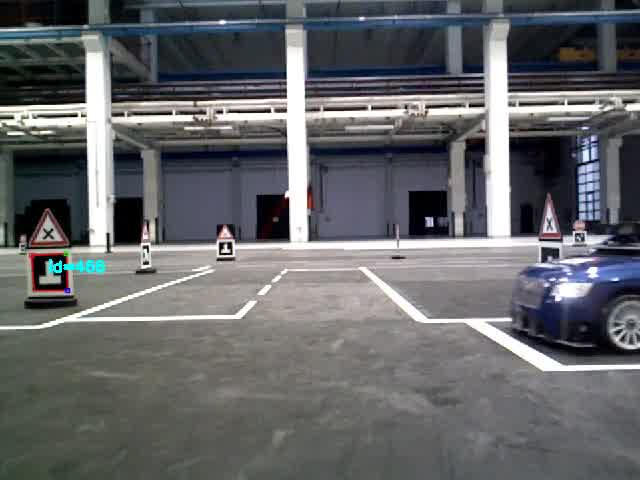
\includegraphics[scale=0.5]{./Abbildungen/bsp1.jpg}
	\caption{Beispiel 1}
	\label{img:bsp1}
\end{figure}

\begin{figure}[p]
	%\hskip-1.0cm
	\centering
	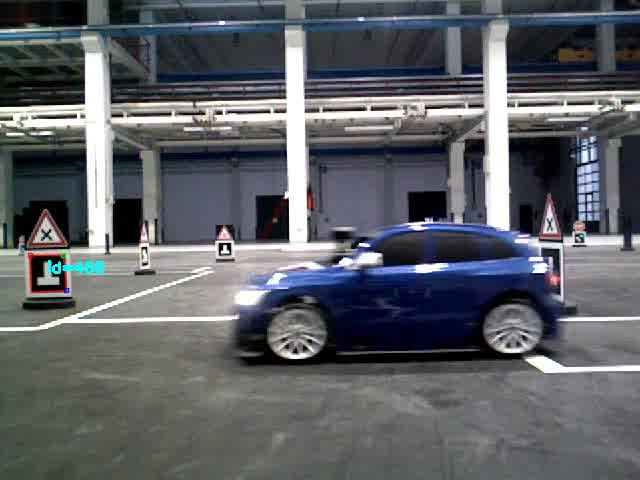
\includegraphics[scale=0.5]{./Abbildungen/bsp2.jpg}
	\caption{Bewegung zu Beispiel 1}
	\label{img:bsp2}
\end{figure}


\section{Aufruf über Kommandozeile}

Damit das Plugin über die Kommandozeile aufgerufen werden kann, muss man es mindestens einmal über \textbf{Compile and Run\dots} ausführen. Daraufhin kann man es über folgenden Befehl aufrufen:

\code{ImageJ -macro /flowig/macro/runplug.ijm Flowig\#path=<dir>,flow=<flowType>}


Parameter:

\code{dir} ist der Ordner, der die Bildfolge enthält.

\code{flowType} stellt den Typ der Berechnung des optischen Flusses dar, es können folgenden Typen angegeben werden:

\begin{itemize}
\item SparseToDense
\item FarneBack
\item DeepFlow
\item DIS
\item DualTVL1
\end{itemize}

\code{showx} und \code{showy}

Ist keine grafische Oberfläche erwünscht, so ist \code{-macro} durch \code{-batch} zu ersetzen.


\chapter{Bewegungserkennung}

%TODO Verfahren erläutern
In diesem Kapitel soll das genutzte Verfahren zur Erkennung von Bewegungen in Bildfolgen erläutert werden.

Das Plugin sucht zunächst nach den Bounding-Boxen. Hierzu werden alle magentafarbene Punkte der Bilder zu Bounding-Boxen zusammengefasst.

Daraufhin \dots

\chapter{title}.